\section{Моделирование и его результаты}
	В данном разделе приводится краткое описание программной реализации
	модели, примеры рассчитанных частотных сканов, примеры результатов
	идентификации их моделей и график зависимости коэффициента 
	нелинейности"=неэкспоненциальности $p$ от расстояния между крайними
	линиями на спектре.

	\subsection{Реализация модели}
	Модель (выражение \ref{eq:dls82e_model_S_p}) реализована на 
	языке программирования Python (версия 3.9.12) с применением 
	библиотеки TensorFlow (версия 2.8.0) и других библиотек	для научных
	вычислений.

	Модель частотного скана реализованна в виде отдельного класса \\
	\emph{FrequencyScan()} в модуле \emph{fsmodels.py}. Код 
	прокомментирован. Все параметры снабжены адекватными значениями по 
	умолчанию. В дальнейшем планируется дополнение документации и 
	перенос всех программных инструментов для обработки 
	экспериментальных данных в один пакет.

	Модель реализует две функции:
	\begin{enumerate}
		\item Вычисление частотного скана по заданным параметрам и 
		заданному вектору десятичных логарифмов частот опорной функции.
		\item Идентификация параметров модели частотного скана по 
		экспериментальным данным.
	\end{enumerate}
	Имеется возможность вывода значений параметров модели на каждой 
	итерации при идентификации. Примеры использования модели можно найти
	в файле \emph{tensorflow\_model.ipynb} (ПО Jupyter Notebook в составе 
	дистрибутива Anaconda).

	Программа при каждом вычислении значения $\phi\left(\tau,F_0,
	t_1\right)$	(выражение~\ref{eq:dls82e_model_phi}) находит 
	\(
		\max{\left[
	    \tau F_0 e^{-\frac{0.05}{\tau F_0}}
	    \left(1-e^{\frac{t_1 F_0-0.45}{\tau F_0}}
	    -e^{-\frac{0.5}{\tau F_0}}+
	    e^{\frac{t_1 F_0-0.95}{\tau F_0}}\right)
	    \right]}
    \)
	методом	градиентного спуска и вычисляет масштабный множитель $M$ 
	(выражение \ref{eq:dls82e_model_M}).

	Идентификация параметров модели производится методом градиетного 
	спуска, при этом минимизируется среднеквадратическая ошибка между 
	значениями, полученными в результате измерений, и результатами 
	моделирования (выражение \ref{eq:mse}).
	\begin{equation}
		\label{eq:mse}
		E = \frac{1}{n}\sum_{i=1}^{n}\left(y_i - y_i^*\right)^2,
	\end{equation}
	где
	\begin{description}
		\item[$y_i$] -- значения, полученные в результате измерений,
		\item[$y_i^*$] -- значения, полученные в результате моделирования,
		\item[$n$] -- количество измерений.
	\end{description}

	Градиентный спуск везде реализован с помощью библиотеки TensorFlow,
	которая использует алгоритм дифференцирования на графе вычислений,
	таким образом, производная берётся символьно (точно), затем вычисляется
	её значение, поэтому точность вычисления градиента ограничена только
	разрядностью чисел \cite{hands_on_ml}.

	\textbf{Для ускорения процесса идентификации и улучшения сходимости
	в модели вместо постоянной времени сигнала релаксации $\tau$ 
	выполняется идентификация величины $\rho = \log_{10}(\tau)$. По этим же
	и некоторым	другим техническим причинам при вычислении частотного 
	скана на вход модели нужно подавать не вектор частот опорной 
	функции, а вектор их десятичных логарифмов.}

	На рисунке \ref{pic:identification_test} показан пример результата
	идентификации модели на тестовых (специально сгенерированных) данных.

	\begin{figure}[h!]
		\centering
		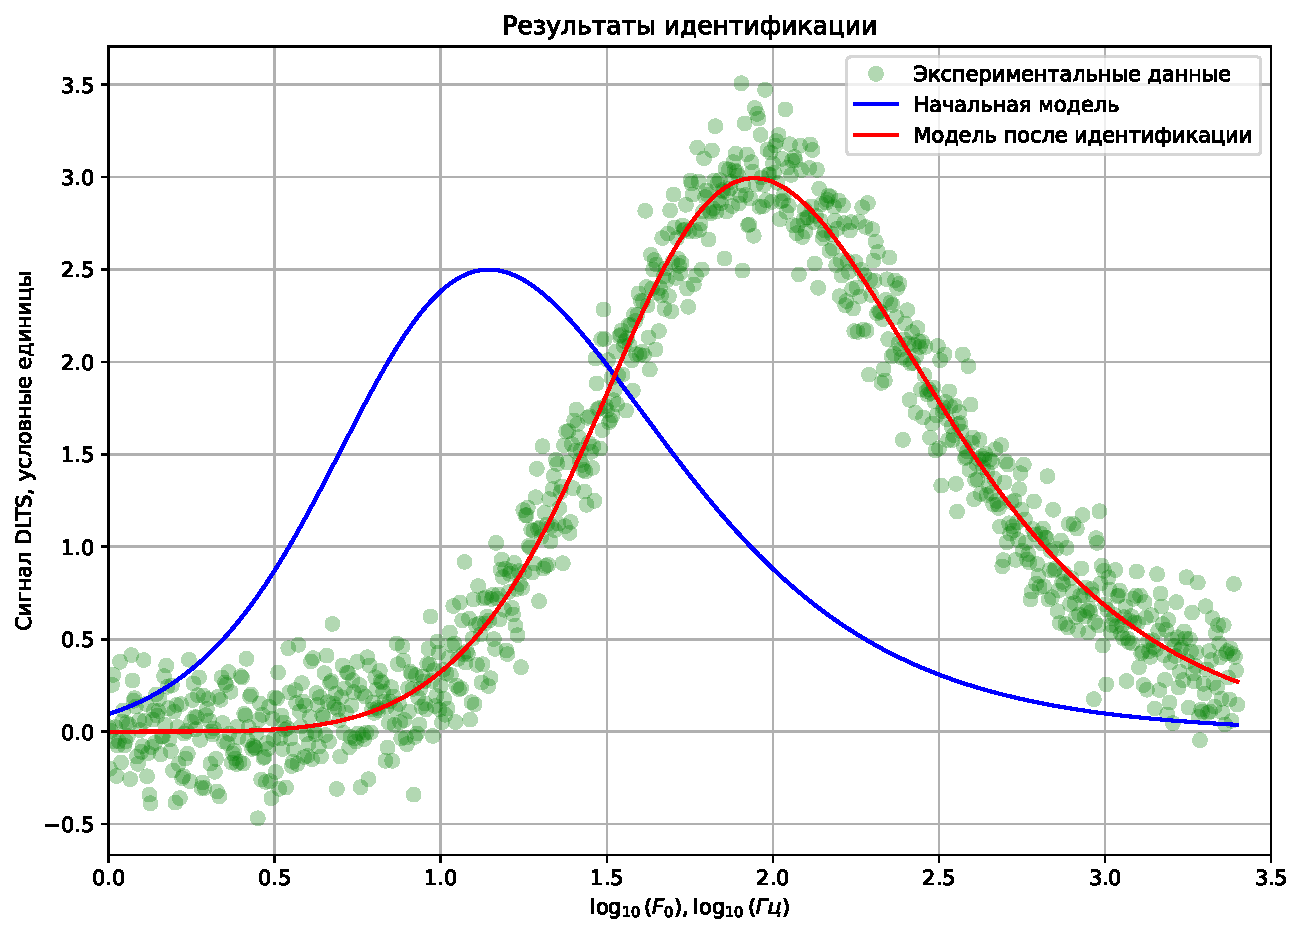
\includegraphics[width=0.75\textwidth]{identification_test}
		\caption{Пример результата идентификации модели.}
		\label{pic:identification_test}
	\end{figure}

	На рисунке \ref{pic:param_path} показан <<путь>> изменеия параметров 
	(десятичного логарифма постоянной времени и амплитуды) при
	идентификации. Красными точками отмечены значения параметров на 
	каждой итерации, изолинии показывают значения среднеквадратической
	ошибки. 

	В идеальном случае изолинии должны иметь форму концентрических
	окружностей, а <<траекторя>> значений параметров должна быть прямой
	линией (в случае обычного градиентного спуска), направленной к центру
	данных окружностей. Таким образом, рисунок \ref{pic:param_path} 
	позволяет сделать вывод о возможности повышения скорости идентификации.

	\begin{figure}[h!]
		\centering
		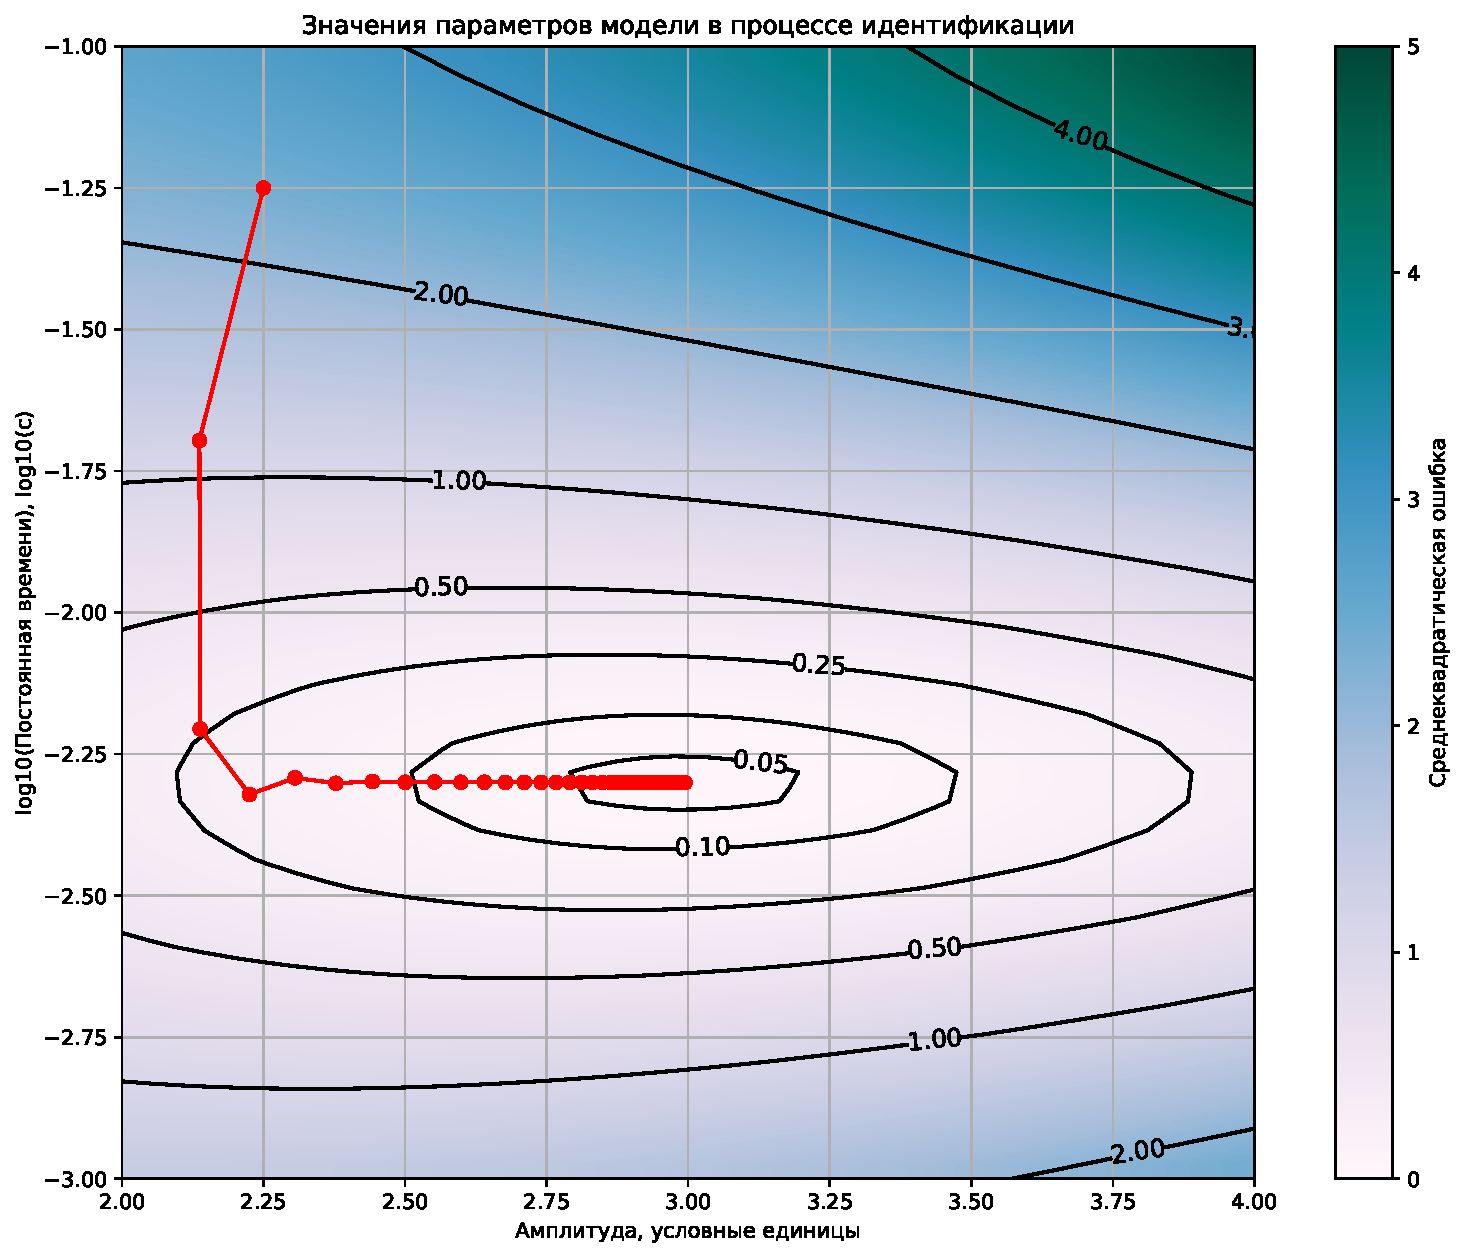
\includegraphics[width=0.75\textwidth]{path}
		\caption{<<Путь>> значений параметров при идентификации.}
		\label{pic:param_path}
	\end{figure}


	\subsection{Результаты моделирования}

	Для определения формы зависимости показателя 
	нелинейности"=неэкспоненциальности $p$ было вы полнено моделирование 
	31 частотного скана со спектрами, состоящими из трёх экспоненциальных
	составляющих единичной амплитуды. При моделировании предполагалось,
	что условия идеальны и частотные сканы не содержат шума.

	На первом этапе моделирования, соглассно выражению \ref{eq:multiexp_frequncy_scan},
	рассчитывался частотный скан, затем производилась идентификация 
	параметров модели этого частотного скана, согласно выражению 
	\ref{eq:dls82e_model_S_p}. Идентификация проводилась по всем точкам.

	Результаты моделирования некоторых частотных сканов и спектры, по 
	которым эти частотные сканы были рассчитаны, приведены на рисунках~
	\ref{pic:result_0},	\ref{pic:result_1}, \ref{pic:result_2}. 
	В таблице~\ref{table:results}, вынесенной в приложение приведены 
	полные результаты моделирования. На рисунке~\ref{pic:p_delta_tau} 
	показан график полученной зависимости показателя	
	нелинейности"=неэспоненциальности от разности постоянных времени
	крайних на спектре линий.

	\begin{figure}[h!]
		\centering
		\begin{subfigure}[c]{0.3\textwidth}
			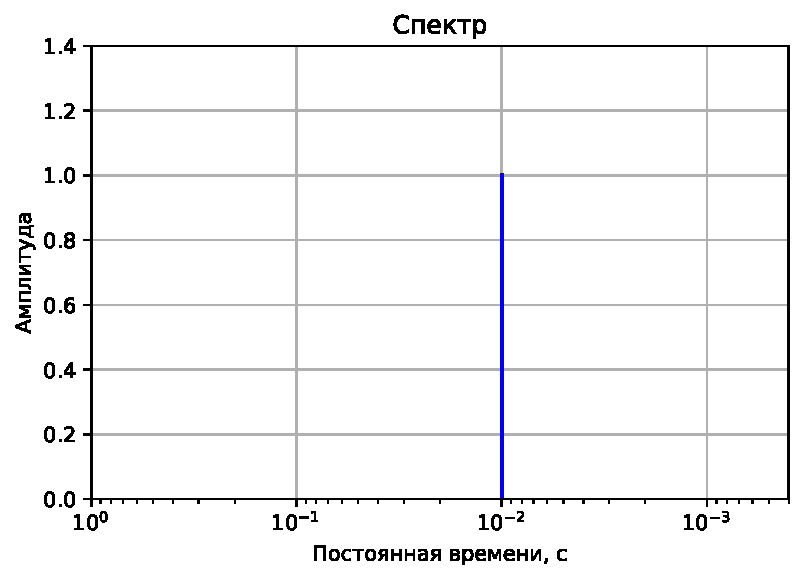
\includegraphics[width=\linewidth]{spectr0}
			\caption{Спектр}
			\label{pic:results_0_spectr}
		\end{subfigure}
		\begin{subfigure}[c]{0.4\textwidth}
			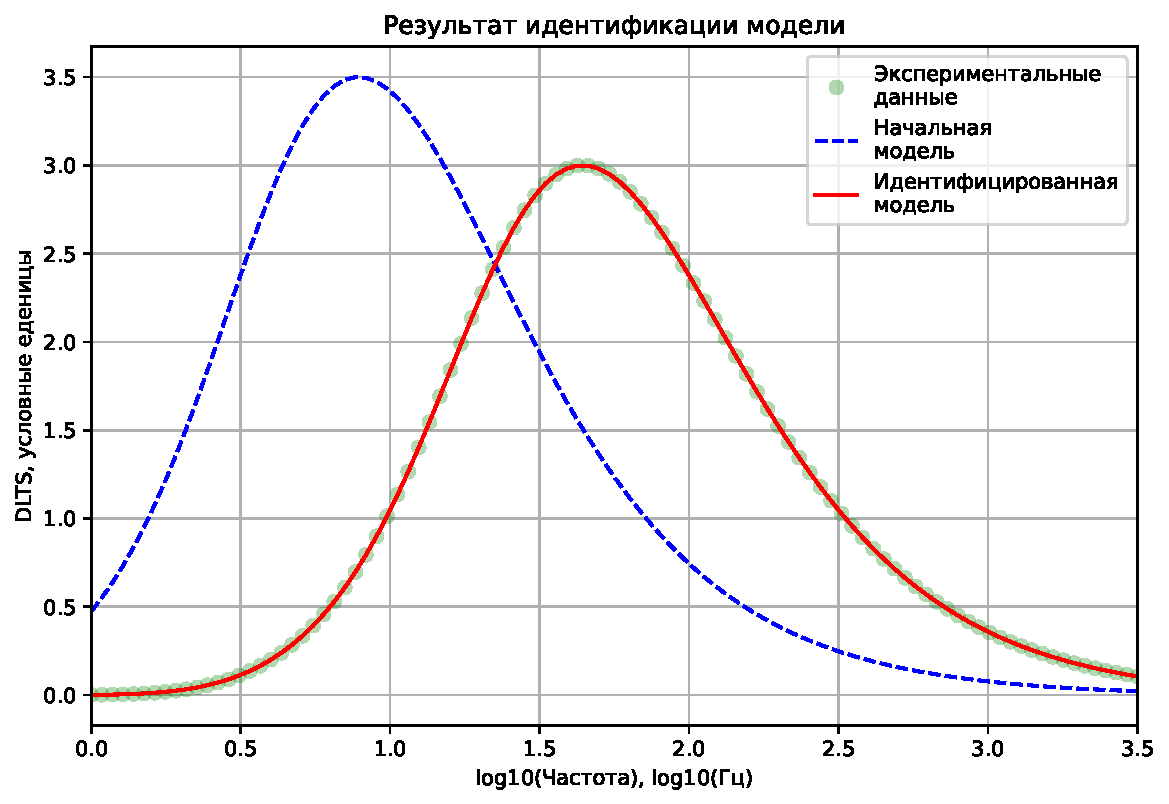
\includegraphics[width=\linewidth]{identification_results_0}
			\caption{Рассчитанный частотный скан и результаты идентификации}
			\label{pic:results_0_scan}
		\end{subfigure}
		\caption{Результаты моделирования частотного скана №1}
		\label{pic:result_0}
	\end{figure}

	\begin{figure}[h!]
		\centering
		\begin{subfigure}[c]{0.3\textwidth}
			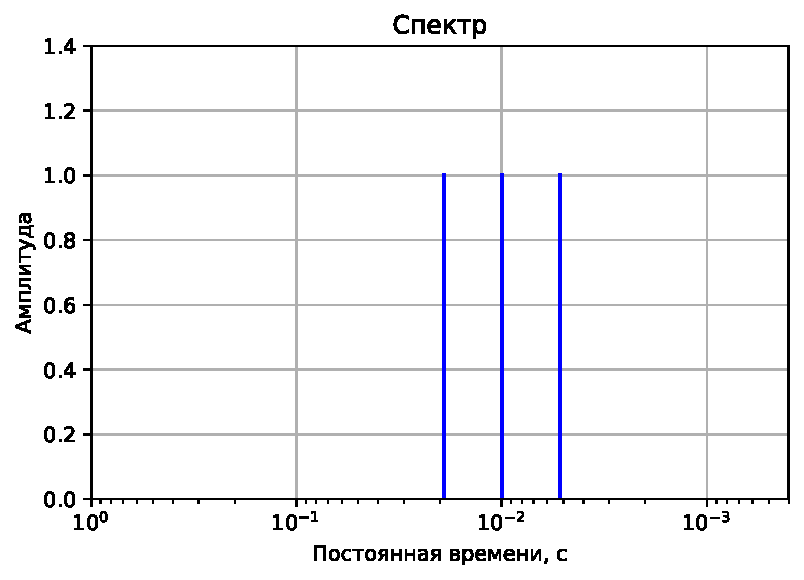
\includegraphics[width=\linewidth]{spectr17}
			\caption{Спектр}
			\label{pic:results_1_spectr}
		\end{subfigure}
		\begin{subfigure}[c]{0.4\textwidth}
			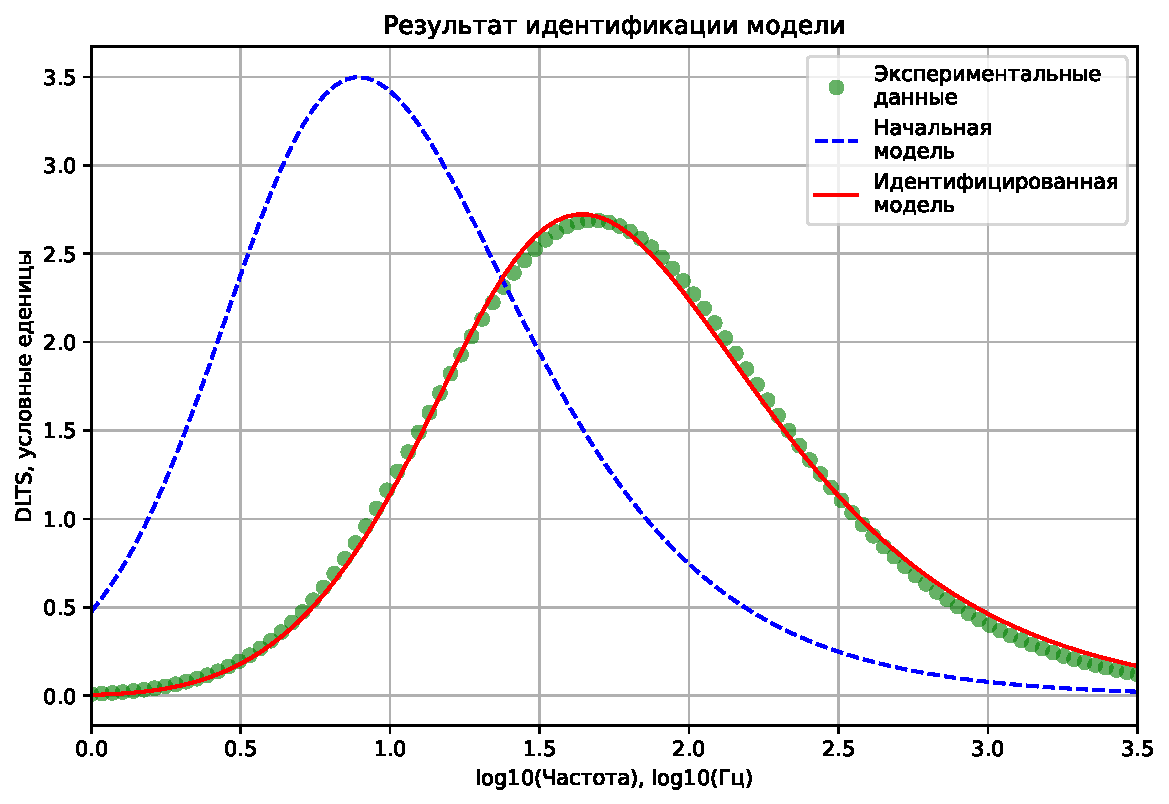
\includegraphics[width=\linewidth]{identification_results_17}
			\caption{Рассчитанный частотный скан и результаты идентификации}
			\label{pic:results_1_scan}
		\end{subfigure}
		\caption{Результаты моделирования частотного скана №18}
		\label{pic:result_1}
	\end{figure}

	\begin{figure}[h!]
		\centering
		\begin{subfigure}[c]{0.3\textwidth}
			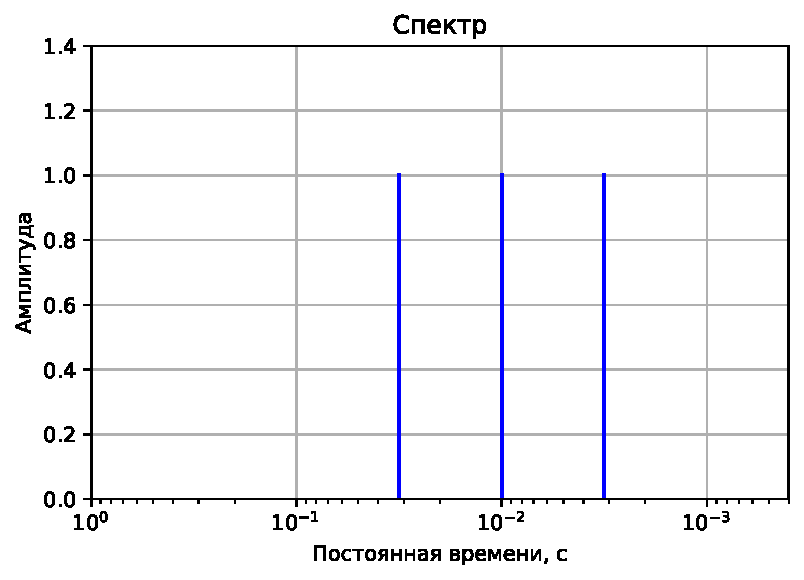
\includegraphics[width=\linewidth]{spectr30}
			\caption{Спектр}
			\label{pic:results_2_spectr}
		\end{subfigure}
		\begin{subfigure}[c]{0.45\textwidth}
			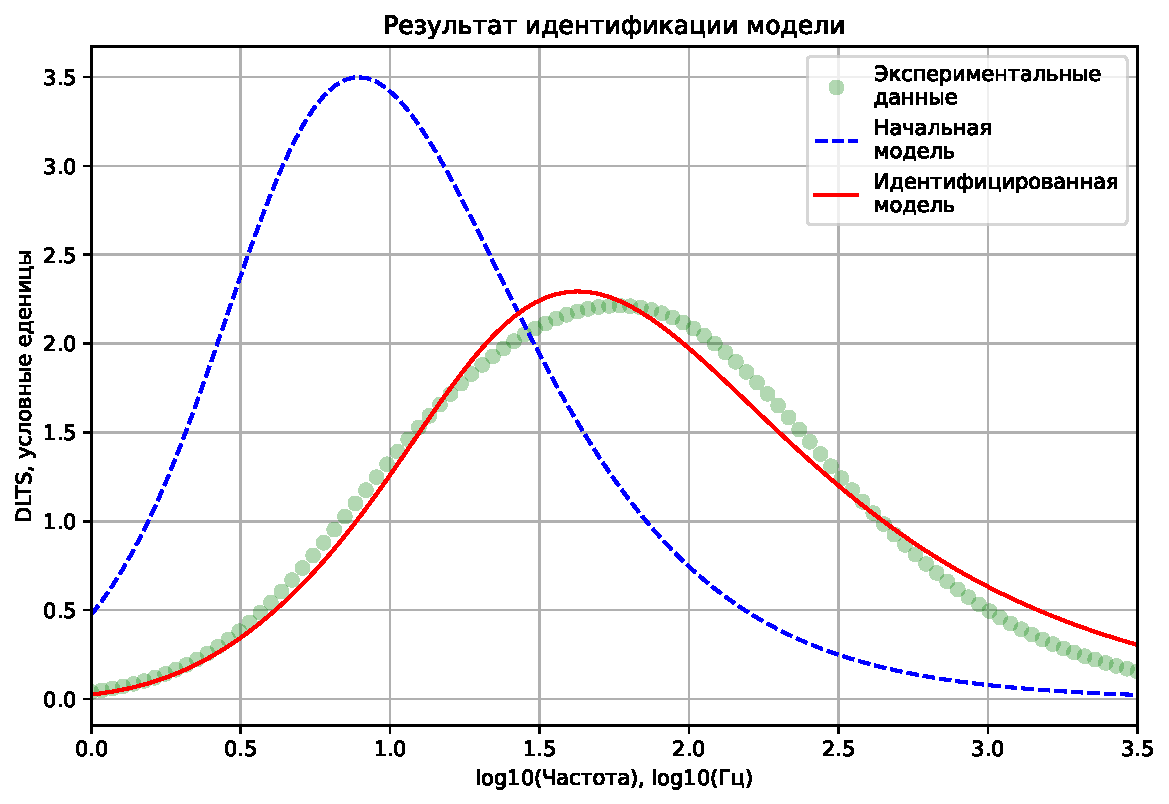
\includegraphics[width=\linewidth]{identification_results_30}
			\caption{Рассчитанный частотный скан и результаты идентификации}
			\label{pic:results_2_scan}
		\end{subfigure}
		\caption{Результаты моделирования частотного скана №31}
		\label{pic:result_2}
	\end{figure}

	\begin{figure}[h!]
		\centering
		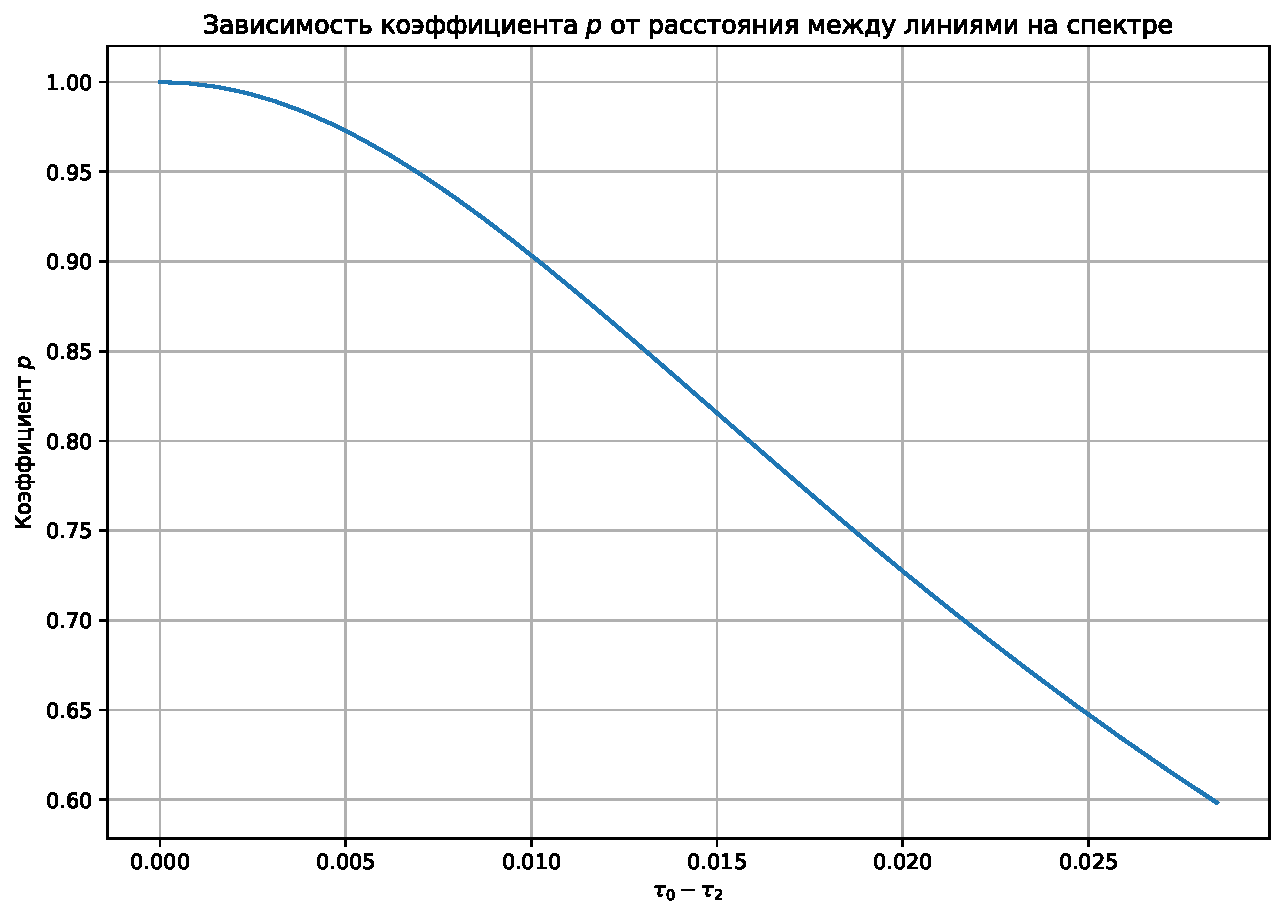
\includegraphics[width=0.7\textwidth]{semilogx_p_func}
		\caption{Зависимость показателя $p$ от разности постоянных времени
		крайних на спектре линий.}
		\label{pic:p_delta_tau}
	\end{figure}